\documentclass{article}
\usepackage[utf8x]{inputenc}
\usepackage{ucs}
\usepackage{amsmath} 
\usepackage{amsfonts}
\usepackage{marvosym}
\usepackage{wasysym}
\usepackage{upgreek}
\usepackage[english,russian]{babel}
\usepackage{graphicx}
\usepackage{float}
\usepackage{textcomp}
\usepackage{hyperref}
\usepackage{geometry}
  \geometry{left=2cm}
  \geometry{right=1.5cm}
  \geometry{top=1cm}
  \geometry{bottom=2cm}
\usepackage{tikz}
\usepackage{ccaption}
\usepackage{multicol}
\usepackage{fancyvrb}

\usepackage{listings}
%\setlength{\columnsep}{1.5cm}
%\setlength{\columnseprule}{0.2pt}

\usepackage{colortbl,graphicx,tikz}
\definecolor{X}{rgb}{.5,.5,.5}

\date{}
\begin{document}
\pagenumbering{gobble}

\lstset{
  language=C++,                % choose the language of the code
  basicstyle=\linespread{1.1}\ttfamily,
  columns=fixed,
  fontadjust=true,
  basewidth=0.5em,
  keywordstyle=\color{blue}\bfseries,
  commentstyle=\color{gray},
  stringstyle=\ttfamily\color{orange!50!black},
  showstringspaces=false,
  %numbers=false,                   % where to put the line-numbers
  numbersep=5pt,
  numberstyle=\tiny\color{black},
  numberfirstline=true,
  stepnumber=1,                   % the step between two line-numbers.        
  numbersep=10pt,                  % how far the line-numbers are from the code
  backgroundcolor=\color{white},  % choose the background color. You must add \usepackage{color}
  showstringspaces=false,         % underline spaces within strings
  captionpos=b,                   % sets the caption-position to bottom
  breaklines=true,                % sets automatic line breaking
  breakatwhitespace=true,         % sets if automatic breaks should only happen at whitespace
  xleftmargin=.2in,
  extendedchars=\true,
  keepspaces = true,
}
\lstset{literate=%
   *{0}{{{\color{red!20!violet}0}}}1
    {1}{{{\color{red!20!violet}1}}}1
    {2}{{{\color{red!20!violet}2}}}1
    {3}{{{\color{red!20!violet}3}}}1
    {4}{{{\color{red!20!violet}4}}}1
    {5}{{{\color{red!20!violet}5}}}1
    {6}{{{\color{red!20!violet}6}}}1
    {7}{{{\color{red!20!violet}7}}}1
    {8}{{{\color{red!20!violet}8}}}1
    {9}{{{\color{red!20!violet}9}}}1
    {~} {$\sim$}{1}
}

\title{Семинар \#2: Инкапсуляция. Домашнее задание.\vspace{-5ex}}\date{}\maketitle

\section*{Класс Circle}
Допустим, что мы хотим создать программу, которая будет работать с окружностями (это может быть игра или, например, графический редактор). Для того, чтобы сделать код более понятным и удобным в использовании, мы решили создать класс окружности. Кроме того, мы решили использовать уже ранее написанный класс точки в 2D пространстве (файлы \texttt{point.h} и \texttt{point.cpp}). Создайте класс окружности, который будет включать следующие методы:
\begin{itemize}
\item Конструктор \texttt{Circle(const Point\& acenter, float aradius)}, который будет задавать поля \texttt{center} и \texttt{radius} соответстующими значениями.
\item Конструктор по умолчанию \texttt{Circle()} - задаются значения, соответствующие единичной окружности с центром в начале координат.
\item Конструктор копирования \texttt{Circle(const Circle\& circle)}
\item Сеттеры и геттеры, для полей \texttt{center} и \texttt{radius}. Поле \texttt{radius} нельзя задать отрицательным числом. При попытке задания его отрицательным числом оно должно устанавливаться в значение \texttt{0}.
\item Метод \texttt{float getArea() const}, который будет возвращать площадь поверхности круга.
\item Метод \texttt{float getDistance(const Point\& p) const}, который будет возвращать расстояние от точки \texttt{p}, до ближайшей точки окружности.
\item Метод \texttt{bool isColliding(const Circle\& c) const}, который будет возвращать \texttt{true}, если круг пересекается с кругом \texttt{c}.
\item Метод \texttt{void move(const Point\& p)}, который будет перемещать кружок на вектор \texttt{p}.
\end{itemize}
Весь начальный код содержится в папке \texttt{0circle}. При компиляции нужно указывать все \texttt{.cpp} файлы, которые вы хотите скомпилировать:
\begin{verbatim}
g++ main.cpp point.cpp
\end{verbatim}
\begin{itemize}
\item Создайте файлы \texttt{circle.h} и \texttt{circle.cpp} и перенесите реализацию класса окружности из файла \texttt{main.cpp} в эти файлы.
\end{itemize}


\newpage
\section*{Класс Number (большое число)}
Стандартные целочисленные  типы данных, такие как \texttt{int} имеют фиксированный небольшой размер. Соответственно значения, которые можно хранить в переменных этих типов ограничены. Типичное максимальное значение \texttt{char} равно $2^7 - 1 = 127$, тип \texttt{int} обычно ограничен $2^{31}-1 = 2147483647$ и даже тип \texttt{unsigned long long} имеет ограничение в $2^{64}-1 = 1.8 * 10^{19}$. Хранить действительно большие числа в этих типах невозможно. В этом задании нужно сделать класс, с помощью которого будет удобно складывать и умножать большие целые положительные числа. Начальный код этого класса содержится в \texttt{1number/number.cpp}. Изучите этот код.


\begin{figure}[h!]
  \centering
  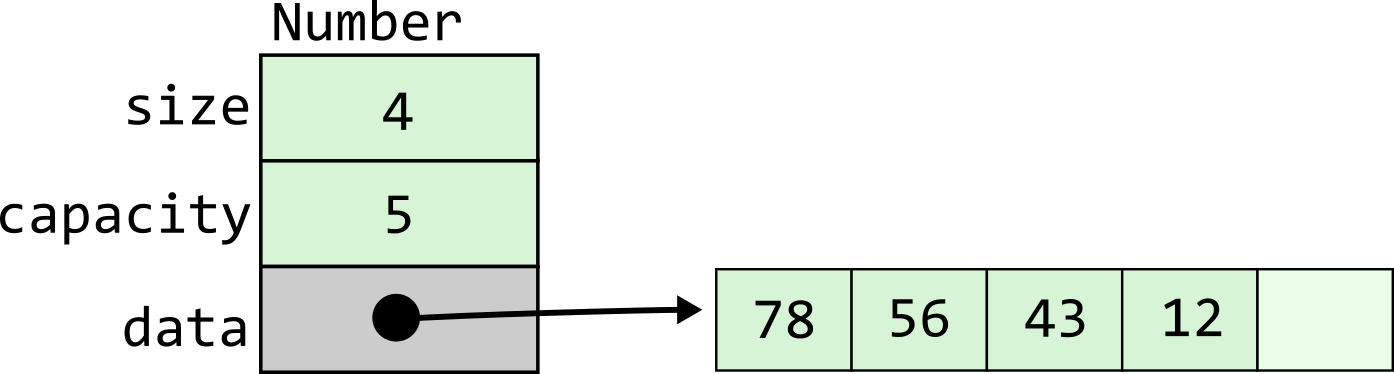
\includegraphics[scale=1]{../images/number1.png}
  \caption{Представление числа 12345678 в памяти с помощью нашего класса Number}
  \label{fig:nummber1}
\end{figure}


\subsection*{Задания:}
\begin{itemize}
\item \textbf{Конструктор по умолчанию:} Напишите конструктор по умолчанию \texttt{Number()}, который будет создавать число равное нулю.
\item \textbf{Конструктор копирования:} Напишите конструктор копирования \texttt{Number(const Number\& n)}.
\item \textbf{Конструктор из строки:} Напишите конструктор \texttt{Number(const char* str)}, который будет создавать большое число на основе строки. Предполагаем, что на вход конструктору всегда идёт корректная строка. Например, число из примера можно будет создать так:
\begin{lstlisting}
Number a = Number("12345678");
\end{lstlisting}
\item \textbf{Присваивание:} Напишите оператор присваивания \texttt{Number\& operator=(const Number\& right)}.
\item \textbf{Сложение:} Напишите и протестируйте операторы сложения \texttt{operator+} и оператор присваивания сложения \texttt{operator+=}.  Реализовывать оба этих оператора с нуля необязательно. Ведь, если написан один из этих операторов, то очень просто написать другой.
\item \textbf{Числа Фибоначчи:} Числа Фибоначчи задаются следующим образом:
\begin{align*}
F_0 &= 0\\
F_1 &= 1\\
F_n &= F_{n-1} + F_{n-2}
\end{align*}
Используйте класс \texttt{Number}, чтобы вычислить $F_{1000}$. Правильный ответ:
\begin{verbatim}
F(1000) = 43466557686937456435688527675040625802564660517371780402481729089536555417949051890
40387984007925516929592259308032263477520968962323987332247116164299644090653318793829896964992
8516003704476137795166849228875
\end{verbatim}




\item \textbf{Четность:} Напишите метод \texttt{bool isEven() const}, который будет проверять является ли наше число чётным и, если это верно, возвращает \texttt{true}, в ином случае возвращает \texttt{false}.

\item \textbf{Произведение:} Напишите метод \texttt{Number operator*(const Number\& right) const} - оператор умножения одного числа \texttt{Number} на другое. Протестируйте вашу функцию на различных примерах (умножение большого числа на большое, умножение большого числа на небольшое ($< 100$) или на ноль, умножение двух небольших чисел и т. д.).\\
\item \textbf{Факториал:} Используйте написанный оператор для вычисления факториала от 1000. \\
Правильный ответ:
\begin{verbatim}
1000! = 40238726007709377354370243392300398571937486421071463254379991042993851239862902059
2044208486969404800479988610197196058631666872994808558901323829669944590997424504087073759
9188236277271887325197795059509952761208749754624970436014182780946464962910563938874378864
8733711918104582578364784997701247663288983595573543251318532395846307555740911426241747434
9347553428646576611667797396668820291207379143853719588249808126867838374559731746136085379
5345242215865932019280908782973084313928444032812315586110369768013573042161687476096758713
4831202547858932076716913244842623613141250878020800026168315102734182797770478463586817016
4365024153691398281264810213092761244896359928705114964975419909342221566832572080821333186
1168115536158365469840467089756029009505376164758477284218896796462449451607653534081989013
8544248798495995331910172335555660213945039973628075013783761530712776192684903435262520001
5888535147331611702103968175921510907788019393178114194545257223865541461062892187960223838
9714760885062768629671466746975629112340824392081601537808898939645182632436716167621791689
0977991190375403127462228998800519544441428201218736174599264295658174662830295557029902432
4153181617210465832036786906117260158783520751516284225540265170483304226143974286933061690
8979684825901254583271682264580665267699586526822728070757813918581788896522081643483448259
9326604336766017699961283186078838615027946595513115655203609398818061213855860030143569452
7224206344631797460594682573103790084024432438465657245014402821885252470935190620929023136
4932734975655139587205596542287497740114133469627154228458623773875382304838656889764619273
8381490014076731044664025989949022222176590433990188601856652648506179970235619389701786004
0811889729918311021171229845901641921068884387121855646124960798722908519296819372388642614
8396573822911231250241866493531439701374285319266498753372189406942814341185201580141233448
2801505139969429015348307764456909907315243327828826986460278986432113908350621709500259738
9863554277196742822248757586765752344220207573630569498825087968928162753848863396909959826
2809561214509948717012445164612603790293091208890869420285106401821543994571568059418727489
9809425474217358240106367740459574178516082923013535808184009699637252423056085590370062427
1243416909004153690105933983835777939410970027753472000000000000000000000000000000000000000
0000000000000000000000000000000000000000000000000000000000000000000000000000000000000000000
0000000000000000000000000000000000000000000000000000000000000000000000000000000000000000000
0000000000000000000000000000
\end{verbatim}

\item \textbf{Числа-градины:} Возьмём некоторое число $n$ и будем последовательно применять к нему следующую функцию:
\begin{equation*}
f(n) = 
    \begin{cases}
      n / 2,   &\textup{если n - четное}\\ 
      3 n + 1, &\textup{если n - нечетное}
    \end{cases}
\end{equation*}
В результате получится некоторая последовательность. Например, при $n = 7$ получится:
\begin{verbatim}
7 -> 22 -> 11 -> 34 -> 17 -> 52 -> 26 -> 13 -> 40 -> 20 -> 10 -> 5 -> 16 -> 8 -> 4 -> 2 -> 1
\end{verbatim}
Последовательность доходит до 1. Вам нужно написать функцию, которая будет по начальному числу находить длину такой последовательности (\texttt{steps}) и максимальное число в этой последовательности(\texttt{max}). Например, для числа $7$, максимальное число в последовательности будет равно $52$, а длина последовательности -- $16$. Напишите программу, которая будет по начальному числу находить длину последовательности и максимальный элемент в ней.

Тесты для проверки:
\begin{verbatim}
n = 7                    steps = 16;      max = 52
n = 256                  steps = 8;       max = 256
n = 1117065              steps = 527;     max = 2974984576
n = 4761963248413673697  steps = 2337;    max = 9926927712374950744648

n = 90560792656972947582439785608972465789628974587264056284658721771
steps = 1630;     
max = 773658021643749360792171137214151494851244403993540980838080564520
\end{verbatim}
Для решения этой задачи нужно написать оператор сравнения и метод деления на 2 (оператор целочисленного деления можно не писать). 
\item \textbf{Раздельная компиляция:} Перенесите объявление класса \texttt{Number} в файл \texttt{number.h}, а определение методов в файл \texttt{number.cpp}. Раздельно скомпилируйте эту программу.
\end{itemize}

\end{document}